\documentclass[fleqn]{homework}

\student{Stephen Brennan (smb196)}
\course{EECS 440}
\assignment{Written Homework 2}
\duedate{September 8, 2015}

\usepackage{mathtools}
\usepackage{amsfonts}
\usepackage{graphicx}

\begin{document}
  \maketitle

  \begin{problem}{1}
    \begin{question}
      Suppose $f$ and $g$ are two convex functions defined on $\mathbb{R}^n$.
      Show that the following functions are also convex: (i)
      $h(x) = f(x) + g(x)$, (ii) $h(x) = \max{(f(x), g(x))}$.  Is
      $h(x) = f(x) - g(x)$ also convex?  Explain why or why not. (10 points)
    \end{question}

    A function is convex iff Jensen's inequality applies to it.

    For (i):
    \begin{align*}
      h(\lambda x_1 + (1 - \lambda) x_2) &= f(\lambda x_1 + (1 - \lambda) x_2) + g(\lambda x_1 + (1 - \lambda) x_2)\\
                                         &\leq \lambda f(x_1) + (1-\lambda)f(x_2) + \lambda g(x_1) + (1-\lambda)g(x_2)\\
                                         &\leq \lambda (f(x_1)+g(x_1)) + (1-\lambda)(f(x_2)g(x_2))\\
                                         &\leq \lambda h(x_1) + (1 - \lambda)h(x_2)\\
    \end{align*}

    Therefore, $h(x) = f(x) + g(x)$ is convex.

    For (ii):
    \begin{align*}
      h(\lambda x_1 + (1 - \lambda) x_2)
      &= \max{f(\lambda x_1 + (1 - \lambda) x_2), g(\lambda x_1 + (1 - \lambda) x_2)}\\
    \end{align*}

    Assume without loss of generality that
    $f(\lambda x_1 + (1 - \lambda) x_2) \geq g(\lambda x_1 + (1 - \lambda)
    x_2)$.  Then, we have:

    \begin{align*}
      h(\lambda x_1 + (1 - \lambda)x_2)
      &= f(\lambda x_1 + (1 - \lambda) x_2) \\
      &\leq \lambda f(x_1) + (1-\lambda) f(x_2) \\
      &\leq \lambda \max{(f(x_1),g(x_1))} + (1-\lambda)\max{(f(x_2), g(x_2))} \\
      &\leq \lambda h(x_1) + (1-\lambda)h(x_2)
    \end{align*}

    Therefore, $h(x) = \max{(f(x), g(x))}$ is convex.

    (iii) No, $h(x)=f(x)-g(x)$ is not necessarily convex.  As a counter-example,
    consider $f(x)=x^2$ and $g(x)=2x^2$.  Both functions are convex, but
    $h(x)=-x^2$, which is not convex.
  \end{problem}

  \begin{problem}{2}
    \begin{question}
      Show that the set $C=\{\vec{x}|A\vec{x} \geq \vec{b}\}$,
      $A \in \mathbb{R}^{m \times n}$, $\vec{x} \in \mathbb{R}^n$,
      $\vec{b} \in \mathbb{R}^m$, is a convex set.  Note that this describes the
      constraint set of a linear program. (10 points)
    \end{question}

    Assume $\vec{x_1}$ and $\vec{x_2}$ are members of $C$.  Therefore,
    $A\vec{x_1} \geq \vec{b}$ and $A\vec{x_2} \geq \vec{b}$.  Any point along
    the line segment connecting $\vec{x_1}$ and $\vec{x_2}$ can be represented
    as $\lambda\vec{x_1} + (1-\lambda)\vec{x_2}$ for $0 \leq \lambda \leq 1$.
    Since
    $A(\lambda\vec{x_1} + (1-\lambda)\vec{x_2}) = \lambda A \vec{x_1} +
    (1-\lambda)A\vec{x_2} \geq \vec{b}$,
    any such point must also be in $C$.  Therefore, $C$ is a convex set.
  \end{problem}

  \begin{problem}{3}
    \begin{question}
      Consider the primal linear program (LP): $\min c^T \vec{x}$ s.t.
      $A\vec{x} \geq \vec{b}, \vec{x} \geq \vec{0}$ and its dual:
      $\max b^T \vec{u}$ s.t. $A^T \vec{u} \leq c, \vec{u} \geq \vec{0}$.
      Carefully prove that for any feasible $(\vec{x},\vec{u})$ (i.e. $\vec{x}$
      and $\vec{u}$ satisfying the constraints of the two LPs),
      $b^T \vec{u} \leq c^T \vec{x}$. (10 points)
    \end{question}

    If $\vec{x}$ and $\vec{u}$ both satisfy the constraints of their respective
    LP's, then we know that $A^T\vec{u} \leq \vec{c}$.  We take the transpose of both
    sides and get:

    \begin{equation*}
      \vec{u}^T A \leq \vec{c}^T
    \end{equation*}

    Now, multiply both sides by $\vec{x}$ on the right, and we get:

    \begin{equation*}
      \vec{u}^T A \vec{x} \leq \vec{c}^T \vec{x}
    \end{equation*}

    Since we know $\vec{b} \leq a \vec{x}$, we can substitute $\vec{b}$ while
    satisfying the inequality:

    \begin{equation*}
      \vec{u}^T \vec{b} \leq \vec{c}^T \vec{x}
    \end{equation*}

    Since $\vec{u}^T \vec{b}$ is a dot product of two vectors, it is the same as
    $\vec{b}^T \vec{u}$.  Substituting, we get the desired inequality:

    \begin{equation*}
      \vec{b}^T \vec{u} \leq \vec{c}^T \vec{x}
    \end{equation*}

  \end{problem}

  \begin{problem}{4}
    \begin{question}
      Prove that the set of all continuous probability distributions over
      $[0,1]$ is convex. (10 points)
    \end{question}

    Let $f$ and $g$ be the density functions of two probability distributions
    over $[0,1]$.  This means that $\int_0^1 f(x) \mathrm{d}x = 1$, and
    similarly for $g$.  For any $h$ defined as
    $h(x) = \lambda f(x) + (1-\lambda) g(x)$, where $0 \leq \lambda \leq 1$, we
    can see that
    $\int_0^1 (\lambda f(x) + (1-\lambda)g(x)) \mathrm{d}x = \lambda\int_0^1
    f(x) \mathrm{d}x + (1-\lambda \int_0^1 g(x)) \mathrm{d}x = 1$.
    Therefore, $h$ is also a continuous probability distribution over $[0,1]$.
  \end{problem}

  \begin{problem}{5}
    \begin{question}
      Consider the LP: $\min c^t \vec{x}$ s.t. $A\vec{x} \geq \vec{b}$,
      $\vec{x} \geq \vec{0}$, where $A$ is the $4 \times 2$ matrix:
      $\begin{bmatrix*} 0 & -1 \\ -1 & -1 \\ -1 & 2 \\ 1 & -1 \end{bmatrix*}$,
      $\vec{b}$ is a $4 \times 1$ vector
      $\begin{bmatrix*} -5 \\ -9 \\ 0 \\ -3 \end{bmatrix*}$, and $\vec{c}$ is a
      $2 \times 1$ vector $\begin{bmatrix*} -1 \\ -2 \end{bmatrix*}$.  (a) Draw
      the feasible region in $\mathbb{R}^2$.  (b) Draw the contours of
      $c^T \vec{x} = -12$, $c^T \vec{x} = -14$, and $c^T \vec{x} = -16$ and
      determine the solution graphically.  (c) Solve the problem using the
      simplex method.  On your figure, trace the path taken by the simplex
      method as it moves to the solution. (10 points)
    \end{question}
    
    (a) The feasible region is shaded below.  Constraints from $A$ are colored
    (red, blue, green, and cyan), while constraints $x,y > 0$ are black.

    \begin{center}
      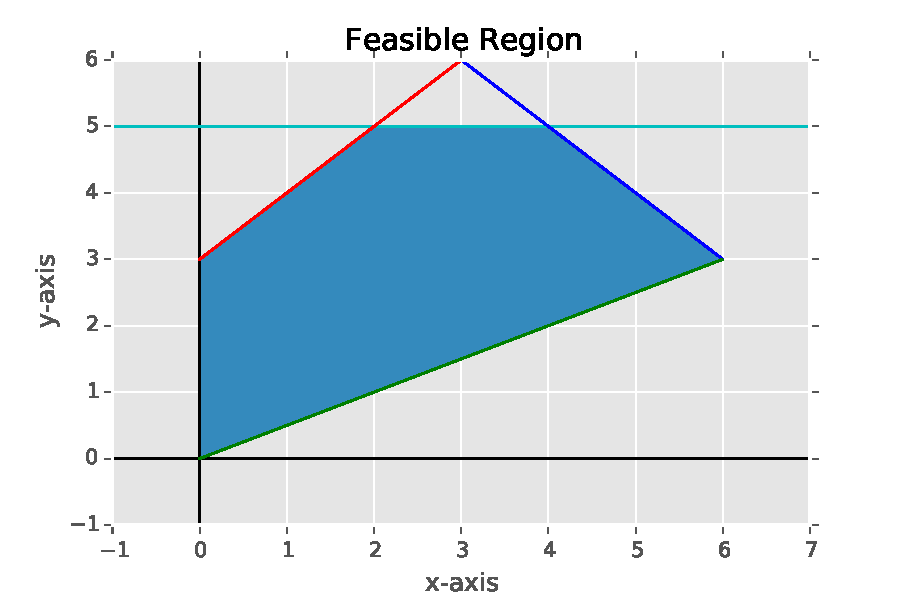
\includegraphics[width=0.7\textwidth]{feasible2.pdf}
    \end{center}

    (b) Below is the modified figure, with the contours in yellow (the lowest is
    $c^T \vec{x} = -12$.  As can be seen, the solution is $(4, 5)$, with a value
    of $-14$.

    \begin{center}
      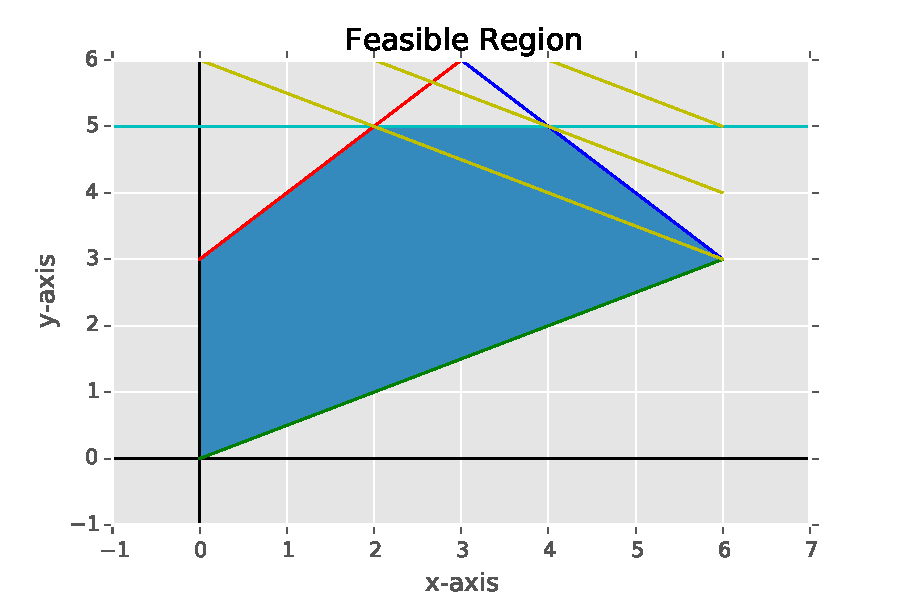
\includegraphics[width=0.7\textwidth]{feasibleb.pdf}
    \end{center}

    (c) The constraints $A \vec{x} \geq \vec{b}$ correspond to the following
    inequalities, and therefore slack variables:

    \begin{align*}
      -y &\geq -5 & w_1 &= -y + 5\\
      -x - y &\geq -9 & w_2 &= -x - y + 9 \\
      -x + 2y &\geq 0 & w_3 &= -x + 2y \\
      x - y &\geq -3 & w_3 &= x - y + 3 \\
    \end{align*}

    This leads to the following initial tableu (at the point $(0,0)$):

    \begin{tabular}{r|rrr}
      & $x$ & $y$ & \\
      \hline
      $w_1$ &  0 & -1 &  5 \\
      $w_2$ & -1 & -1 &  9 \\
      $w_3$ & -1 &  2 &  0 \\
      $w_4$ &  1 & -1 &  3 \\
      $z$   & -1 & -2 &  0 \\
    \end{tabular}

    $y$ will decrease the objective function the most, so we pick it.  We find
    that the blocking constraint comes from $w_4$, and it sets $y=3$.  So we
    swap $y$ and $w_4$ in the tableau, getting the following (at the point
    $(0, 3)$):

    \begin{tabular}{r|rrr}
      & $x$ & $w_4$ & \\
      \hline
      $w_1$ & -1 &  1 &  2 \\
      $w_2$ & -2 &  1 &  6 \\
      $w_3$ &  1 & -2 &  6 \\
      $y$   &  1 & -1 &  3 \\
      $z$   & -3 &  2 & -6 \\
    \end{tabular}

    Next we choose $x$.  The blocking constraint comes from $w_1$, and sets
    $x=2$.  So, we swap $x$ and $w_1$, getting the following (at the point
    $(2, 5)$):

    \begin{tabular}{r|rrr}
      & $w_1$ & $w_4$ & \\
      \hline
      $x$   & -1 &  1 &  2 \\
      $w_2$ &  2 & -1 &  2 \\
      $w_3$ & -1 & -1 &  8 \\
      $y$   & -1 &  0 &  5 \\
      $z$   &  3 &  -1 & -12 \\
    \end{tabular}

    Next we choose $w_4$.  The blocking constraint comes from $w_2$, setting
    $w_4 = 2$.  So, we swap $w_4$ and $w_2$, getting the following (at the point
    $(4, 5)$):

    \begin{tabular}{r|rrr}
      & $w_1$ & $w_2$ & \\
      \hline
      $x$   &  1 & -1 &  4 \\
      $w_4$ &  2 & -1 &  2 \\
      $w_3$ & -3 &  1 & -2 \\
      $y$   & -1 &  0 &  5 \\
      $z$   &  1 &  1 & -14 \\
    \end{tabular}

    Since the coefficients of the objective function are now both positive, we
    can no longer decrease it, so the Simplex method is complete.  The solution
    is $(4, 5)$, with $z=-14$.  Below is the figure with the steps above traced
    along it:

    \begin{center}
      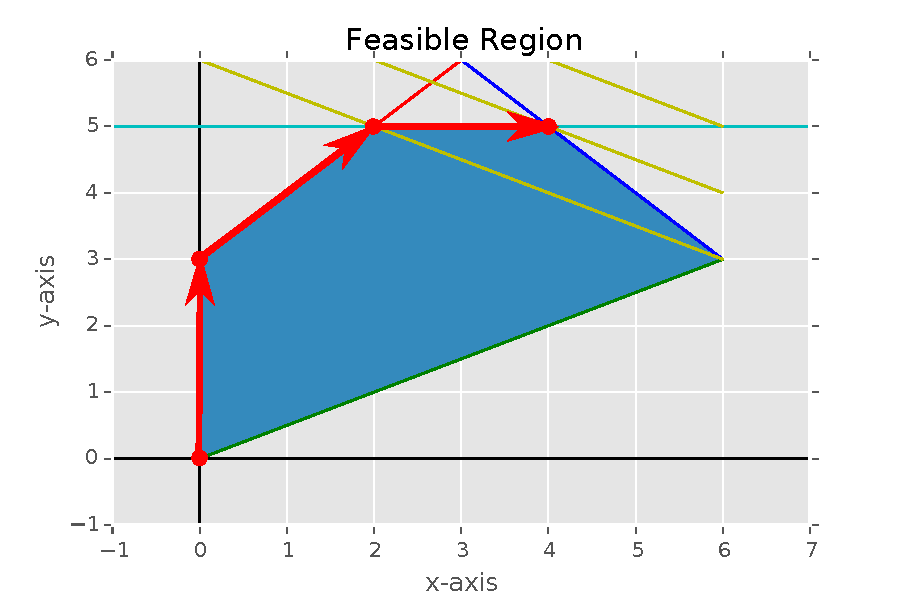
\includegraphics[width=0.7\textwidth]{pathc.pdf}
    \end{center}
  \end{problem}

\end{document}